%###############################################################################
%# WbXbc - Manual - Plain Crossbar Switch                                      #
%###############################################################################
%#    Copyright 2018 Dirk Heisswolf                                            #
%#    This file is part of the WbXbc project.                                  #
%#                                                                             #
%#    WbXbc is free software: you can redistribute it and/or modify            #
%#    it under the terms of the GNU General Public License as published by     #
%#    the Free Software Foundation, either version 3 of the License, or        #
%#    (at your option) any later version.                                      #
%#                                                                             #
%#    WbXbc is distributed in the hope that it will be useful,                 #
%#    but WITHOUT ANY WARRANTY; without even the implied warranty of           #
%#    MERCHANTABILITY or FITNESS FOR A PARTICULAR PURPOSE.  See the            #
%#    GNU General Public License for more details.                             #
%#                                                                             #
%#    You should have received a copy of the GNU General Public License        #
%#    along with WbXbc.  If not, see <http://www.gnu.org/licenses/>.           #
%###############################################################################
%# Version History:                                                            #
%#   October 1, 2018                                                           #
%#      - Initial release                                                      #
%###############################################################################

\subsection[WbXbc Xbar]{WbXbc Xbar (\texttt{WbXbc\_xbar})}
\label{xbar}

This module implements a full crossbar switch between a set of initator
busses and a set of target busses, all using the pipelined Wishbone    
protocol (see \figref{xbar:diag}).                                                              
%      Initiator         Initiator            Initiator   
%          |                 |      . . .        |    
%          V                 V                   V    
% +----------------------------------------------------------------------+
% |        |                 |                   |                       | 
% |        V                 V                   V                       |
% |  +-----------+     +-----------+       +-----------+                 |
% |  |WbXbc      |     |WbXbc      |       |WbXbc      |                 |
% |  |Distributor|     |Distributor| . . . |Distributor|                 |
% |  +-+-+-----+-+     +-+-+-----+-+       +-+-+-----+-+                 |
% |    | | ... |         | | ... |           | | ... |                   |
% |    | |     |         | |     |           | |     |                   |
% |    | |     |         | |     |           | |     |     +---------+   |       
% |    +-|-----|---------|-|-----|-----------|-|-----|---->|         |   |       
% |      |     |         +-|---- |-----------|-|-----|---->| WbXbc   +-->|-->Target
% |      |     |           |     |           | |     | ... | Arbiter |   |       
% |      |     |           |     |           +-|-----|---->|         |   |       
% |      |     |           |     |             |     |     +---------+   |       
% |      |     |           |     |             |     |                   |       
% |      |     |           |     |             |     |     +---------+   |       
% |      +-----|-----------|-----|-------------|-----|---->|         |   |       
% |            |           +-----|-------------|-----|---->| WbXbc   +-->|-->Target
% |            |                 |             |     | ... | Arbiter |   |       
% |            |                 |             +-----|---->|         |   |       
% |            |                 |                   |     +---------+   |       
% |            |                 |                   |                   |       
% |            |                 |                   |        . . .      |   . . .       
% |            |                 |                   |                   |       
% |            |                 |                   |     +---------+   |       
% |            +-----------------|-------------------|---->|         |   |       
% |                              +-------------------|---->| WbXbc   +-->|-->Target
% |                                                  | ... | Arbiter |   |       
% |     WbXbc                                        +---->|         |   |       
% |     Xbar                                               +---------+   |  
% |                                                                      |
% +----------------------------------------------------------------------+
\begin{figure}[!h]
  %\begin{center}
  \makebox[\textwidth][c]{
    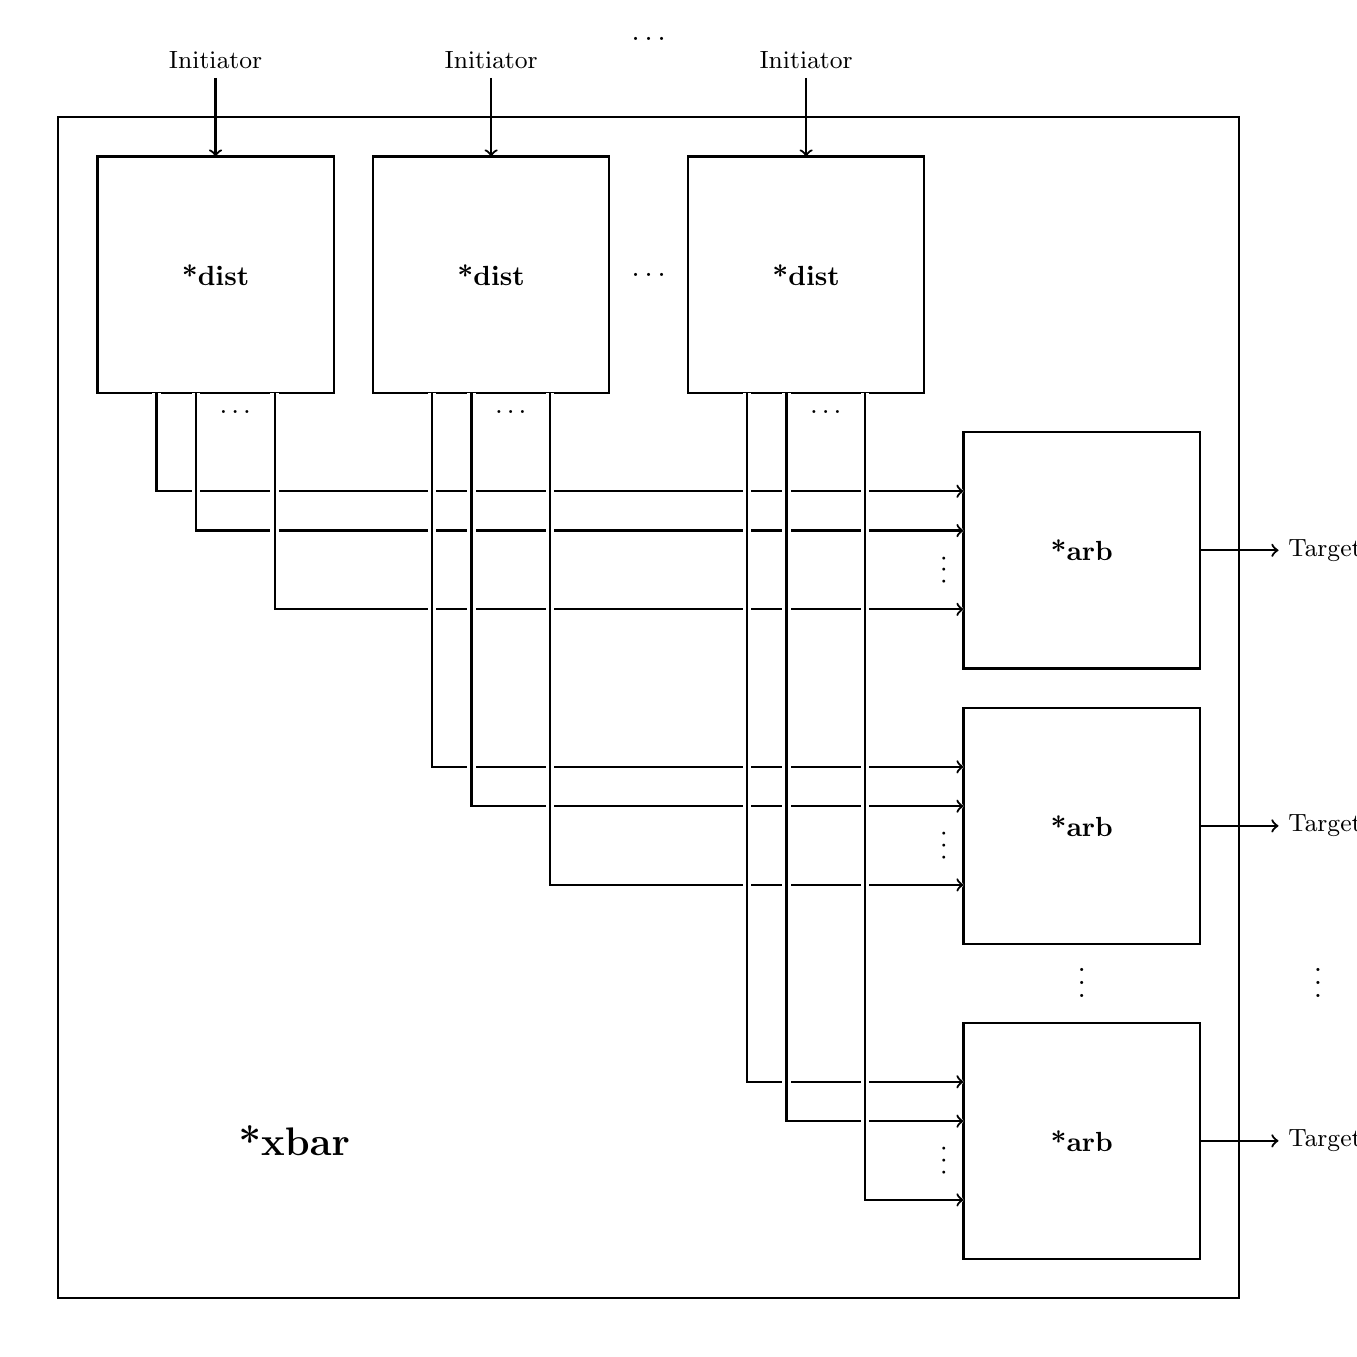
\begin{tikzpicture}
      %Block boundary
      \draw [thick, fill=white] (0,0) rectangle (15,15);
      \node at (3,2)
            {\begin{minipage}[c]{16em}
                \begin{center}
                  \hyphenchar\font=-1
                  \Large{\textbf{\nameref*{xbar}}}
                \end{center}
            \end{minipage}};
      %Distributors
      \newsavebox{\distbox}
      \savebox{\distbox}{
        \draw [thick, fill=white] (0,0) rectangle (3,3);
        \node at (1.5,1.5)
              {\begin{minipage}[c]{8em}
                  \begin{center}
                    \hyphenchar\font=-1
                    \textbf{\nameref*{dist}}
                  \end{center}
              \end{minipage}};
        \node [above] at (1.5,4)
              {\begin{minipage}[c]{4em}
                  \begin{center}
                    \hyphenchar\font=-1
                    \small{Initiator}
                  \end{center}
              \end{minipage}};
        \node at (1.75,-0.25) {\footnotesize{\texttt{...}}};
        \draw [thick, ->] (1.5,4) -- (1.5,3);}
      \node at (0.5,11.5) {\usebox{\distbox}};
      \node at (4,11.5)   {\usebox{\distbox}};
      \node at (7.5,13)   {\small{\texttt{...}}};
      \node at (7.5,16)   {\small{\texttt{...}}};
      \node at (8,11.5)   {\usebox{\distbox}}; 
      %Arbiters
      \newsavebox{\arbbox}
      \savebox{\arbbox}{
        \draw [thick, fill=white] (0,0) rectangle (3,3);
        \node at (1.5,1.5)
              {\begin{minipage}[c]{8em}
                  \begin{center}
                    \hyphenchar\font=-1
                    \textbf{\nameref*{arb}}
                  \end{center}
              \end{minipage}};
        \node [right] at (4,1.5)
              {\begin{minipage}[c]{4em}
                  \begin{flushleft}
                    \hyphenchar\font=-1
                    \small{Target}
                  \end{flushleft}
              \end{minipage}};
        \node [rotate=90] at (-0.25,1.25) {\footnotesize{\texttt{...}}};
        \draw [thick, ->] (3,1.5) -- (4,1.5);}
      \node at (11.5,8)   {\usebox{\arbbox}};
      \node at (11.5,4.5) {\usebox{\arbbox}};
      \node [rotate=90] at (13,4) {\small{\texttt{...}}};
      \node [rotate=90] at (16,4) {\small{\texttt{...}}};
      \node at (11.5,0.5)   {\usebox{\arbbox}};
      %Connections
      \draw [preaction={draw, line width=3pt, white}, thick, ->] ( 1.25,11.5) -- ( 1.25,10.25) -- (11.5,10.25);
      \draw [preaction={draw, line width=3pt, white}, thick, ->] ( 1.75,11.5) -- ( 1.75, 9.75) -- (11.5, 9.75);
      \draw [preaction={draw, line width=3pt, white}, thick, ->] ( 2.75,11.5) -- ( 2.75, 8.75) -- (11.5, 8.75);
             
      \draw [preaction={draw, line width=3pt, white}, thick, ->] ( 4.75,11.5) -- ( 4.75, 6.75) -- (11.5, 6.75);
      \draw [preaction={draw, line width=3pt, white}, thick, ->] ( 5.25,11.5) -- ( 5.25, 6.25) -- (11.5, 6.25);
      \draw [preaction={draw, line width=3pt, white}, thick, ->] ( 6.25,11.5) -- ( 6.25, 5.25) -- (11.5, 5.25);
             
      \draw [preaction={draw, line width=3pt, white}, thick, ->] ( 8.75,11.5) -- ( 8.75, 2.75) -- (11.5, 2.75);
      \draw [preaction={draw, line width=3pt, white}, thick, ->] ( 9.25,11.5) -- ( 9.25, 2.25) -- (11.5, 2.25);
      \draw [preaction={draw, line width=3pt, white}, thick, ->] (10.25,11.5) -- (10.25, 1.25) -- (11.5, 1.25);
             
    \end{tikzpicture}
    }
    \caption{Block Diagram of the \nameref*{xbar}}
    \label{xbar:diag}
  %\end{center}
\end{figure}

\subsubsection{Integration Parameters}
\label{xbar:param}

The \nameref*{xbar} supports the integration parameters listed in \tabref{xbar:param:tab}. 
See \secref{param} for a detailed description of all integration parameters.

\begin{center}
  \rowcolors{1}{gray!12}{white}                                         %set alternating row color
  \begin{longtable}{|l|r|l|}
    \rowcolor{white}
    \caption{Integration Parameters of the \nameref*{xbar}}
    \label{xbar:param:tab} \\
    %Header
    \hline                                     
    \rowcolor{gray!25}
    \multicolumn{1}{|c|}{\textbf{\rule{0pt}{2.5ex} Parameter}}  &  
    \multicolumn{1}{c|}{\textbf{\rule{0pt}{2.5ex}  Default}}    & 
    \multicolumn{1}{c|}{\textbf{\rule{0pt}{2.5ex}  Decription}} \\
    \hline                                    
    \endhead                               
    %Footers
    \hline
    \rowcolor{white}
    \multicolumn{3}{r}{\tiny{...continued}} \\
    \endfoot
    \hline
    \endlastfoot
    %Content
    \texttt{ITR\_CNT   } & \texttt{4}  & Number of initiator busses           \\
    \texttt{TGT\_CNT   } & \texttt{4}  & Number of target busses              \\
    \texttt{ADDR\_WIDTH} & \texttt{16} & Width of the address bus             \\
    \texttt{DATA\_WIDTH} & \texttt{16} & Width of each data bus               \\
    \texttt{SEL\_WIDTH } & \texttt{2}  & Number of data select lines          \\
    \texttt{TGA\_WIDTH } & \texttt{1}  & Number of address tags               \\
    \texttt{TGC\_WIDTH } & \texttt{1}  & Number of cycle tags                 \\
    \texttt{TGRD\_WIDTH} & \texttt{1}  & Number of read data tags             \\
    \texttt{TGWD\_WIDTH} & \texttt{1}  & Number of write data tags            \\
  \end{longtable}
\end{center}

\subsubsection{Interface Signals}
\label{xbar:sig}

\tabref{xbar:sig:tab} lists the interface signals of the \nameref*{xbar}. 
See \secref{sig} for a detailed description of all interface signals.

\begin{center}
  \rowcolors{1}{gray!12}{white}                                         %set alternating row color
  \begin{longtable}{|l|r|l|l|}
    \rowcolor{white}
    \caption{Interface Signals of the \nameref*{xbar}}
    \label{xbar:sig:tab} \\
    %Header
    \hline                                     
    \rowcolor{gray!25}
    \multicolumn{1}{|c|}{\textbf{\rule{0pt}{2.5ex} Signal}}     &  
    \multicolumn{1}{c|}{\textbf{\rule{0pt}{2.5ex}  Range}}      & 
    \multicolumn{1}{c|}{\textbf{\rule{0pt}{2.5ex}  Direction}}  & 
    \multicolumn{1}{c|}{\textbf{\rule{0pt}{2.5ex}  Decription}} \\
    \hline
    \endhead                               
    %Footers
    \hline
    \rowcolor{white}
    \multicolumn{4}{r}{\tiny{...continued}} \\
    \endfoot
    \hline
    \endlastfoot
    %Section 'Clock and Reset'
    %\hline
    \rowcolor{gray!20}
    \multicolumn{4}{|c|}{\scriptsize{\rule{0pt}{2.5ex} Clock and Reset}} \global\rownum=1\relax \\*  
    \nobreakhline                                    
    \texttt{clk\_i}        &                                & input & module clock              \\*
    \texttt{async\_rst\_i} &                                & input & asynchronous reset        \\*
    \texttt{sync\_rst\_i}  &                                & input & synchronous reset         \\
    %Section 'Target Address Regions'
    %\hline
    \rowcolor{gray!20}
    \multicolumn{4}{|c|}{\scriptsize{\rule{0pt}{2.5ex} Target Address Regions}} \global\rownum=1\relax                   \\*  
    \nobreakhline                                    
    \texttt{region\_addr\_i} & \texttt{(TGT\_CNT*ADDR\_WIDTH)\-1:0} & input & target address                             \\*
    \texttt{region\_mask\_i} & \texttt{(TGT\_CNT*ADDR\_WIDTH)\-1:0} & input & \makecell[l]{selects relevant address bits \\*
                                                                                           (1: relevant, 0: ignored)}    \\
    %Section 'Initiator Interface'
    \hline                                 
    \rowcolor{gray!20}
    \multicolumn{4}{|c|}{\scriptsize{\rule{0pt}{2.5ex} Initiator Interface}} \global\rownum=1\relax                    \\*    
    \nobreakhline                                 
    \texttt{itr\_cyc\_i}         & \texttt{ITR\_CNT-1:0}               & input  & concatinated bus cycle indicators    \\*
    \texttt{itr\_stb\_i}         & \texttt{ITR\_CNT-1:0}               & input  & concatinated access requests	       \\*
    \texttt{itr\_we\_i}          & \texttt{ITR\_CNT-1:0}               & input  & concatinated write enables	       \\*
    \texttt{itr\_lock\_i}        & \texttt{ITR\_CNT-1:0}               & input  & concatinated bus cycle locks	       \\*
    \texttt{itr\_sel\_i}         & \texttt{(ITR\_CNT*SEL\_WIDTH)-1:0}  & input  & concatinated write data selects      \\*
    \texttt{itr\_adr\_i}         & \texttt{(ITR\_CNT*ADDR\_WIDTH)-1:0} & input  & concatinated address busses	       \\*
    \texttt{itr\_dat\_i}         & \texttt{(ITR\_CNT*DATA\_WIDTH)-1:0} & input  & concatinated write data busses       \\*
    \texttt{itr\_tga\_i}         & \texttt{(ITR\_CNT*TGA\_WIDTH)-1:0}  & input  & concatinated address tags	       \\*
    \texttt{itr\_tga\_prio\_i}   & \texttt{ITR\_CNT-1:0}               & input  & concatinated access priorities       \\*
    \texttt{itr\_tgc\_i}         & \texttt{(ITR\_CNT*TGC\_WIDTH)-1:0}  & input  & concatinated bus cycle tags	       \\*
    \texttt{itr\_tgd\_i}         & \texttt{(ITR\_CNT*TGWD\_WIDTH)-1:0} & input  & concatinated write data tags	       \\*
    \texttt{itr\_ack\_o}         & \texttt{ITR\_CNT-1:0}               & output & concatinated bus cycle acknowledges  \\*
    \texttt{itr\_err\_o}         & \texttt{ITR\_CNT-1:0}               & output & concatinated error indicators	       \\*
    \texttt{itr\_rty\_o}         & \texttt{ITR\_CNT-1:0}               & output & concatinated retry requests	       \\*
    \texttt{itr\_stall\_o}       & \texttt{ITR\_CNT-1:0}               & output & concatinated access delays	       \\*
    \texttt{itr\_dat\_o}         & \texttt{(ITR\_CNT*DATA\_WIDTH)-1:0} & output & concatinated read data buses	       \\*
    \texttt{itr\_tgd\_o}         & \texttt{(ITR\_CNT*TGRD\_WIDTH)-1:0} & output & concatinated read data tags          \\ 
    %Section 'Target Interface'
    \hline                                                                                      
    \rowcolor{gray!20}
    \multicolumn{4}{|c|}{\scriptsize{\rule{0pt}{2.5ex} Target Interface}} \global\rownum=1\relax                      \\*  
    \nobreakhline                                                                                      
    \texttt{tgt\_cyc\_o}         & \texttt{TGT\_CNT-1:0}               & output & concatinated bus cycle indicators   \\*
    \texttt{tgt\_stb\_o}         & \texttt{TGT\_CNT-1:0}               & output & concatinated access requests	      \\*
    \texttt{tgt\_we\_o}          & \texttt{TGT\_CNT-1:0}               & output & concatinated write enables	      \\*
    \texttt{tgt\_lock\_o}        & \texttt{TGT\_CNT-1:0}               & output & concatinated bus cycle locks	      \\*
    \texttt{tgt\_sel\_o}         & \texttt{(TGT\_CNT*SEL\_WIDTH)-1:0}  & output & concatinated write data selects     \\*
    \texttt{tgt\_adr\_o}         & \texttt{(TGT\_CNT*ADDR\_WIDTH)-1:0} & output & concatinated write data selects     \\*
    \texttt{tgt\_dat\_o}         & \texttt{(TGT\_CNT*DATA\_WIDTH)-1:0} & output & concatinated write data busses      \\*
    \texttt{tgt\_tga\_o}         & \texttt{(TGT\_CNT*TGA\_WIDTH))-1:0} & output & concatinated address tags	      \\*
    \texttt{tgt\_tgc\_o}         & \texttt{(TGT\_CNT*TGC\_WIDTH)-1:0}  & output & concatinated bus cycle tags	      \\*
    \texttt{tgt\_tgd\_o}         & \texttt{(TGT\_CNT*TGWD\_WIDT)-1:0}  & output & concatinated write data tags	      \\*
    \texttt{tgt\_ack\_i}         & \texttt{TGT\_CNT-1:0}               & input  & concatinated bus cycle acknowledges \\*
    \texttt{tgt\_err\_i}         & \texttt{TGT\_CNT-1:0}               & input  & concatinated error indicators	      \\*
    \texttt{tgt\_rty\_i}         & \texttt{TGT\_CNT-1:0}               & input  & concatinated retry requests	      \\*
    \texttt{tgt\_stall\_i}       & \texttt{TGT\_CNT-1:0}               & input  & concatinated access delays	      \\*
    \texttt{tgt\_dat\_i}         & \texttt{(TGT\_CNT*DATA\_WIDTH-1):0} & input  & concatinated read data busses	      \\*
    \texttt{tgt\_tgd\_i}         & \texttt{(TGT\_CNT*TGRD\_WIDTH-1):0} & input  & concatinated read data tags         \\   
  \end{longtable}
\end{center}  

\subsubsection{Verification Status}
\label{xbar:verif}

\tabref[Table]{xbar:verif:tab} provides an overview of the verification status of the \nameref*{xbar}.
Lint checks have been done with the Icarus Verilog simulator~\cite{iverilog} and the Yosys synthesis tool~\cite{yosys}.

\begin{center}
  \rowcolors{1}{gray!12}{white}                                         %set alternating row color
  \begin{longtable}{|lr|c|c|c|c|}
    \rowcolor{white}
    \caption[Interface Signals]{Verification Status of the \nameref*{xbar}}
    \label{xbar:verif:tab} \\
    %Header
    \hline                              
    \rowcolor{gray!25}
    \multicolumn{2}{|c|}{\textbf{\rule{0pt}{2.5ex} Configuration}} &  
    \multicolumn{1}{c|}{\textbf{\rule{0pt}{2.5ex}  Linting}}       &  
    \multicolumn{1}{c|}{\textbf{\rule{0pt}{2.5ex}  Simulation}}    &  
    \multicolumn{1}{c|}{\textbf{\rule{0pt}{2.5ex}  Formal}}        &  
    \multicolumn{1}{c|}{\textbf{\rule{0pt}{2.5ex}  FPGA}}          \\
    \hline                              
    \endhead                               
    %Footers
    \hline
    \rowcolor{white}
    \multicolumn{6}{r}{\tiny{...continued}} \\
    \endfoot
    \hline
    \endlastfoot
    %Content
    \makecell[l]{Default:             \\ 
                 \texttt{ITR\_CNT}    \\
                 \texttt{TGT\_CNT}    \\
                 \texttt{ADDR\_WIDTH} \\
                 \texttt{DATA\_WIDTH} \\
                 \texttt{SEL\_WIDTH}  \\
                 \texttt{TGA\_WIDTH}  \\
                 \texttt{TGC\_WIDTH}  \\
                 \texttt{TGRD\_WIDTH} \\
                 \texttt{TGWD\_WIDTH}}   &
    \makecell[r]{                     \\ 
                 \texttt{4}           \\
                 \texttt{4}           \\
                 \texttt{16}          \\
                 \texttt{16}          \\
                 \texttt{2}           \\
                 \texttt{1}           \\
                 \texttt{1}           \\
                 \texttt{1}           \\
                 \texttt{1}}             &     
    \makecell[c]{iVerilog~\cite{iverilog} \\                    
                 Yosis~\cite{yosys}}     &
    & & \\
  \end{longtable}
\end{center}
  

